\documentclass[english,peerreview]{sareport}
% use the option peerreview for creating an anonymized version of your report
% E.g., \documentclass[english,peerreview]{sareport}

\usepackage[colorlinks, linkcolor=black, citecolor=black, urlcolor=black]{hyperref}
\usepackage{float}


% Set all authors, if your group counts 2, set third author empty \authorthree{}
% Set the groupname as well
\authorone{Robin Haveneers (r0450702)}
\authortwo{Stef Verreydt (r0456110)}
\authorthree{Axel Lemmens (r0462440)}
\groupname{Haveneers-Verreydt-Lemmens}

\academicyear{2016--2017}

\casename{Shared Internet Of Things Infrastructure Platform}
\phasenumber{1}
\phasename{Domain Analysis}


\begin{document}
\maketitle

\tableofcontents

\chapter{Domain analysis}\label{sec:domain}
\section{Domain models}
This sections contains the domain models for our system. For readability reasons, the model is split in two parts. In the first figure the general domain model is shown, in the second figure the model cotaining the hardware and information flow is depicted.

\begin{figure}[H]
    \centering
    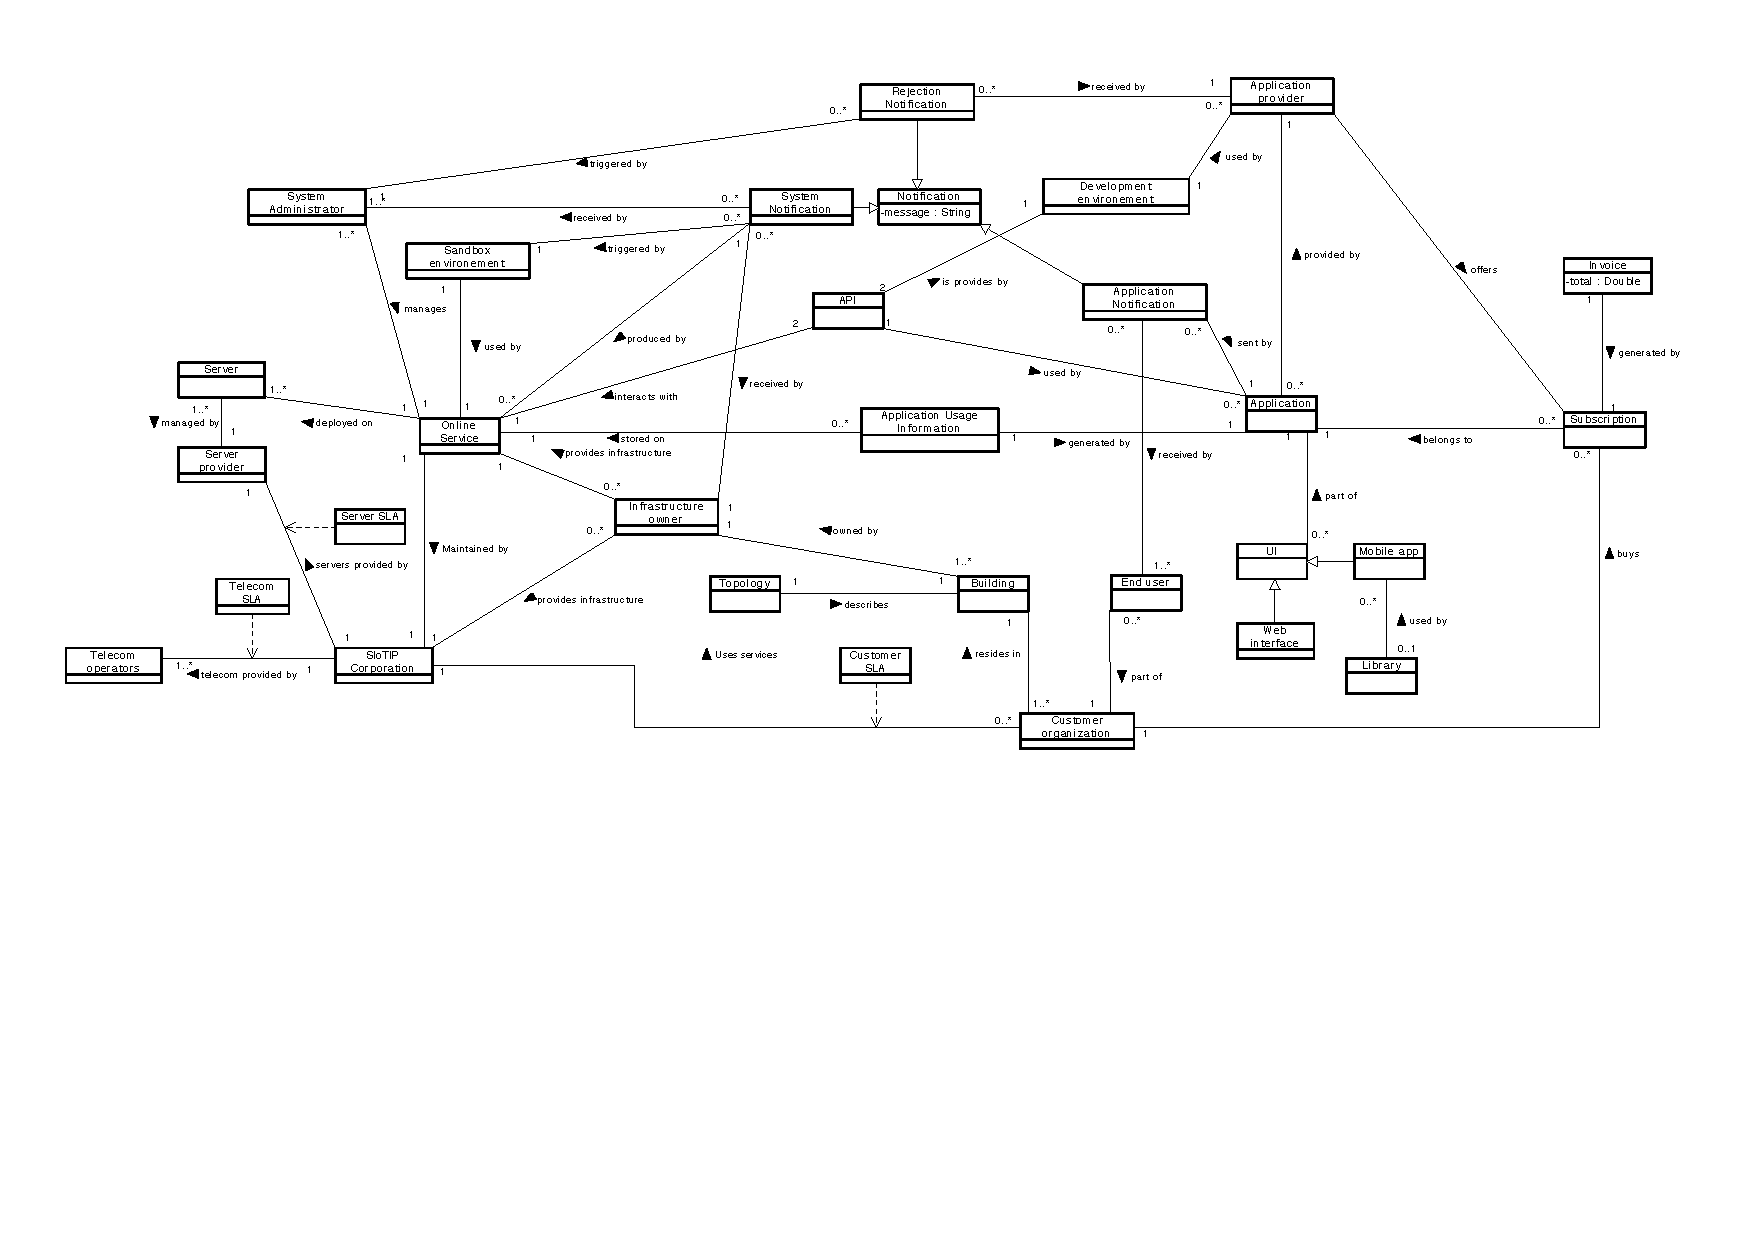
\includegraphics[width=\textwidth, height=9cm, angle=90]{Domain_model.pdf}
    \caption{Domain model: General}\label{fig:domain_model1}
\end{figure}

\begin{figure}[H]
    \centering
    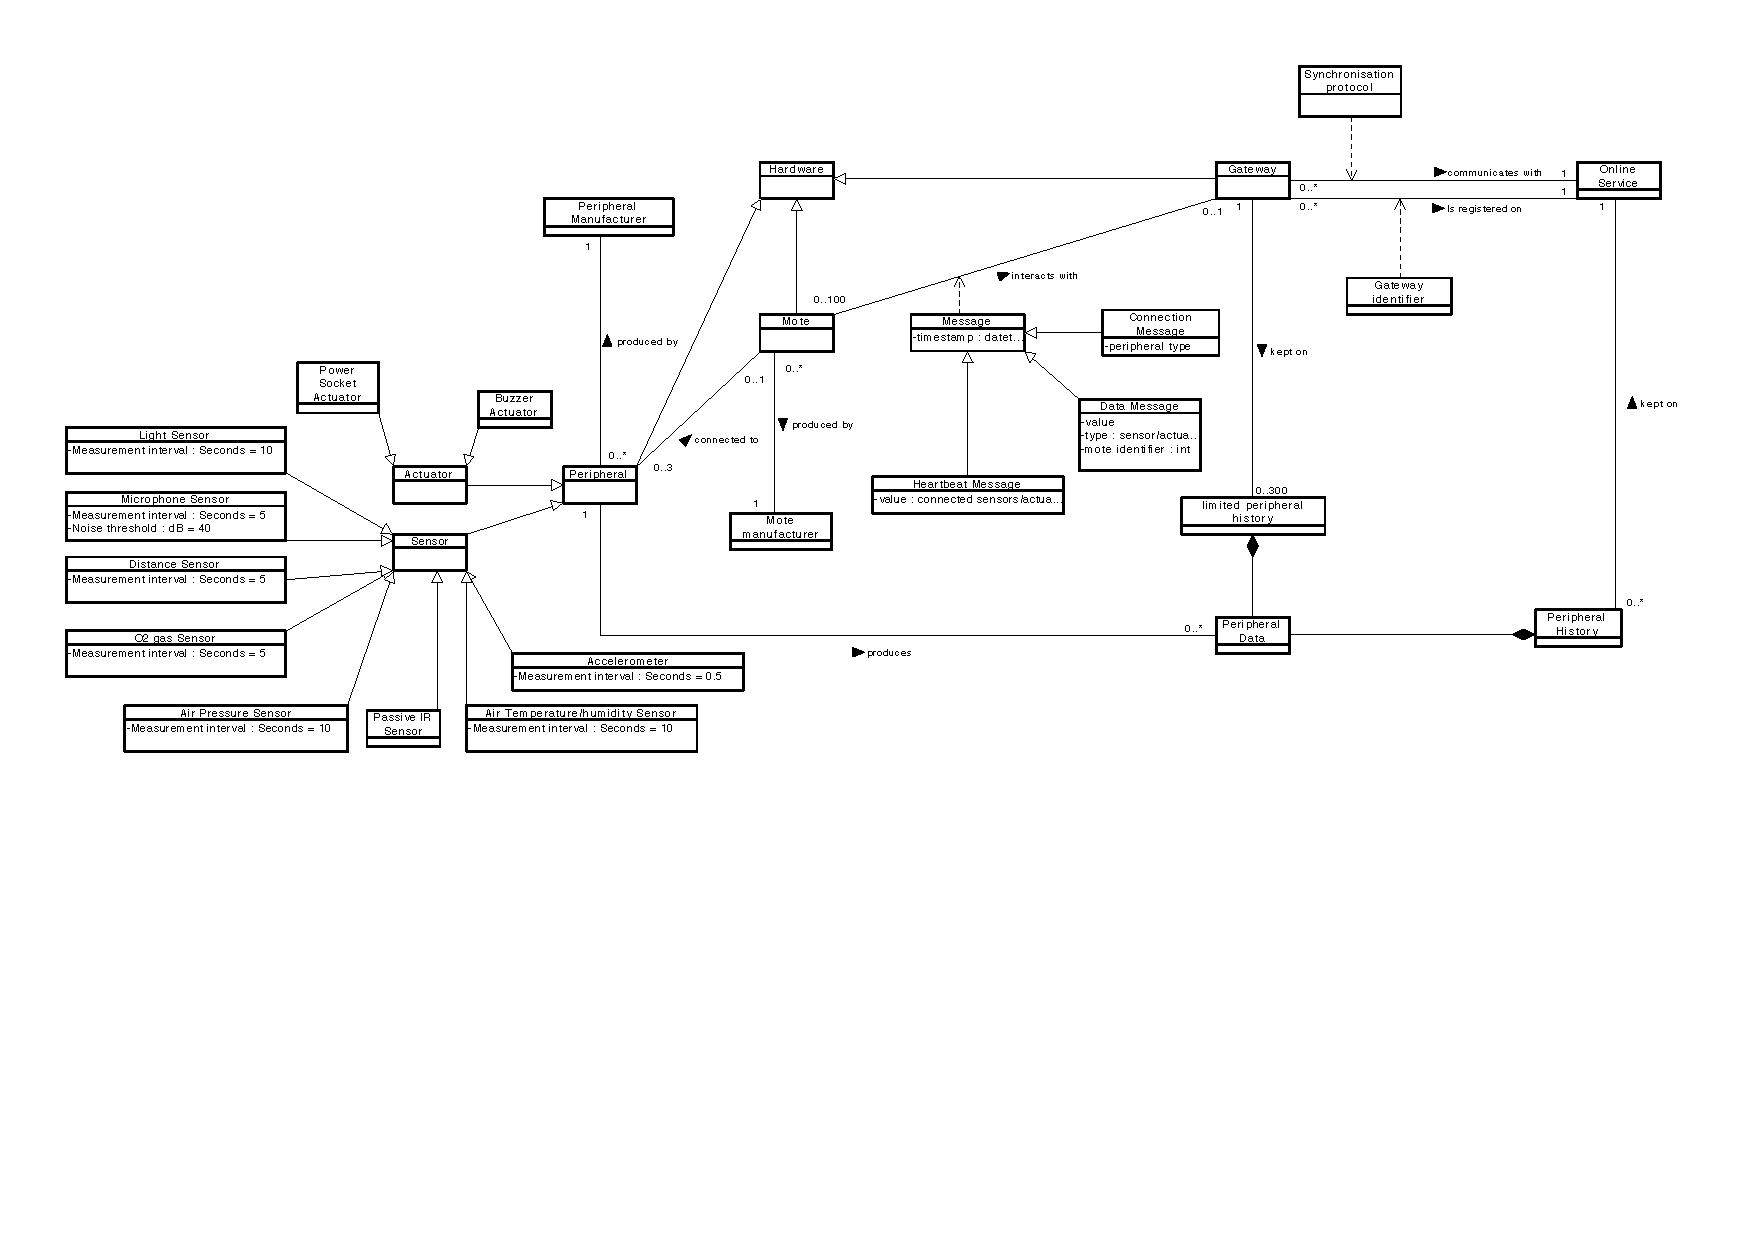
\includegraphics[width=\textwidth, height=9cm, angle=90]{Hardware_and_information_flow.pdf}
    \caption{Domain model: Hardware and information flow}\label{fig:domain_model2}
\end{figure}
\section{Domain constraints}
In this section we provide additional domain constraints.

\begin{itemize}
    \item A customer organization can only subscribe to an application that is already registered with the system.
    \item A end-user only receives notifications from applications that the customer organization he works for is subscribed to. He only receives these notifcations if he/she is an individual who should receive notifications as configured in the application by the previously mentioned customer organization.
    \item The Online Service can only communicate with peripherals via their gateway.
    \item The connectivity between the network manager and the attached devices is done via 6LoWPAN.
    \item Application developers only receive rejection notification about the applications they want to deploy.
    \item An application should be idle until all the necesarry hardware is available and if the hardware is available it should be activated automatically. For example, a fire application requires at least 2 specific sensors per room.
    \item If a component of the hardware fails, the system should automatically switch to a nearby, similar device if possible, based on the topology provided by the infrastructure owner.
    \item Only persons who are allowed to do so, can issue commands to an application.
    \item Gateways contain limited storage space. Whenever they're runnin low on space, the oldest information should be removed.
    \item When communicating with the system, customer organisations, infrastructure owners, system administrators and application providers each have their own, personal, dashboard to do so.
\end{itemize}

\section{Domain constraints}
In this section we provide additional domain constraints.

\begin{itemize}
    \item A customer organization can only subscribe to an application that is already registered with the system.
    \item A end-user only receives notifications from applications that the customer organization he works for is subscribed to. He only receives these notifcations if he/she is an individual who should receive notifications as configured in the application by the previously mentioned customer organization.
    \item The Online Service can only communicate with peripherals via their gateway.
    \item The connectivity between the network manager and the attached devices is done via 6LoWPAN.
    \item Application developers only receive rejection notifications about the applications they want to deploy.
    \item An application should be idle until all the necesarry hardware is available and if the hardware is available it should be activated automatically. For example, a fire application requires at least 2 specific sensors per room.
    \item If a component of the hardware fails, the system should automatically switch to a nearby, similar device if possible, based on the topology provided by the infrastructure owner.
    \item Only persons who are allowed to do so, can issue commands to an application.
    \item Gateways contain limited storage space. Whenever they're runnin low on space, the oldest information should be removed.
    \item When communicating with the system, customer organisations, infrastructure owners, system administrators and application providers each have their own, personal, dashboard to do so.
\end{itemize}

\section{Glossary}
In this section, we provide a glossary of the most important terminology used
in this analysis.

\begin{itemize}
	\item \textbf{API}: Application programming interface. The interface used by applications to communicate with the online system and gateways.
	\item \textbf{Accelerometer}: Type of sensor that measures the acceleration in 3 dimensions.
	\item \textbf{Actuator}: Hardware device that has actions associated with it (e.g. switch, light, buzzer ...)
	\item \textbf{Air Pressure Sensor}: Type of sensor that measures the air pressur in bar.
	\item \textbf{Air Temperature/Humidity Sensor}: Type of sensor the measures the air temperature in degrees Celcius and humidity in percentage.
	\item \textbf{Application Notification}: A type of notification send by the application to a relevant end-user.
	\item \textbf{Application Usage Information}: Data collected by applications and stored on the online service. Useful for providing insight in application usage and big data analytics.
	\item \textbf{Application provider}: Stakeholder that provides (develops and deploys) applications on the online system, to which one can subscribe.
	\item \textbf{Application}: Piece of 'software' running on the online service and gateway provided to customer organizations to subscribe to with the goal of simplifying their day to day business.
	\item \textbf{Building}: Place owned by infrastructure owner where customer organisations are housed. The infrastructure owners keeps a topology about the buidling they own.
	\item \textbf{Buzzer}: Actuator that is able to play a sound.
	\item \textbf{Connection Message}: THe message that is sent by the mote to the gateway whenever a new sensor or actuator is inserted.
	\item \textbf{Customer SLA}: The Service-Level Agreement between SIoTIP corporation and the customer organisation.
	\item \textbf{Customer organization}: The stakeholder in our system which subscribes to applications which optimize their workflow.
	\item \textbf{Data Message}: The message send by the mote from one of its connected devices to the gatewy which contains the value it's reading, the mote identifier and a timestamp. This message also specifies whether it was sent by a sensor/actuator which is necessary to be able to correctly interpret the data.
	\item \textbf{Development environement}: The environmennt available to application providers to freely test and debug their application before deploying it.
	\item \textbf{Distance Sensor}: Type of sensor which measure 
	\item \textbf{End user}: A person involved in the customer organisation who interacts with applications.
	\item \textbf{Gateway identifier}: The identifier which is used to register the gateway with the Online Service.
	\item \textbf{Gateway}: A device that is connected to the online service and which provides access to sensors and actuators. It relays data from connected devices to the Online Service.
	\item \textbf{Hardware}: Umbrella concept used for all the connected devices (such as peripherals, gateways ...)
	\item \textbf{Heartbeat Message}: Periodical message sent by the mote to indicate it is alive. This message includes a list of connected sensors and actuators as well as a timestamp indicating when the message was generated.
	\item \textbf{Infrastructure owner}: Stakeholder in our system which manages the physical infrastructure as well as the hardware used as described in the toplogy. Customer organisations reside in these buidlings.
	\item \textbf{Invoice}: An invoice is associated with a subscription between a customer organization and an application provider. It specifies the fees necessary to be paid by the customer organization.
	\item \textbf{Library}: Set of methods that can be used by application providers in their mobile applications to simplify development.
	\item \textbf{Light Sensor}: Type of sensor that measures the amount of light in LUX.
	\item \textbf{Llimited peripheral history}: Small set of peripheral history maintained by the gateway. Useful for application to, for example, learn certain behavourial patterns.
	\item \textbf{Message}: Umbrella term used for the different types of messages a mote can emit.
	\item \textbf{Microphone Sensor}: Type of sensor which allows detection of sound. 
	\item \textbf{Mobile app}: One type of interface end-users can use to communicate with the online system.
	\item \textbf{Mote manufacturer}: Third party which produces the motes used by our system.
	\item \textbf{Mote}: Device that hosts sensors and actuators.
	\item \textbf{Notification}: Umbrella concept used for all the different types of notifications used by the system. Notifications are sent out on several events. The precise information depends on the type of event.
	\item \textbf{O$_2$ gas sensor}: Sensor that can measure the amount of O$_2$ gas in the air  in percentage.
	\item \textbf{Online Service}: The collective concept that are the services provided via our online back-end. This service is used to test, develop and host applications, to store application configurations, keep track of sensor data, collect usage statistics etc. 
	\item \textbf{Passive IR (Presence) Sensor}: Type of sensor which allows detection of motion achieved by taking pictures and comparing subsequent pictures.
	\item \textbf{Peripheral Data}: The data which is produced by peripherals/hardware. Hardwa
	\item \textbf{Peripheral History}
	\item \textbf{Peripheral Manufacturer}: The third party company that is responsible for the manufacturing of sensors and actuators.
	\item \textbf{Peripheral Type}: The type of the peripheral. Currently sensor and actuator are possible.
	\item \textbf{Peripheral}: Umbrella concept for sensors and actuators.
	\item \textbf{Power socket}: Type of actuator which can be turned on or off.
	\item \textbf{Rejection Notification}: The type of notification which is triggered by the sandbox environment if the application that is waiting to be deployed is rejected by our system. This notification is send to the application provider.
	\item \textbf{SIoTIP Corporation}: This stakeholder wants SIoTIP to be a succesful platform for deploying IoT devices. They have agreements with different third parties for providing an optimal platform with respect to availability, performance ..
	\item \textbf{Sandbox environement}: The environment which is used to test submitted applications before they become available on the Online Service. When there are problems with the application being tested, a system admininstrator performs a secondary, manual review. If he rejects the application, the application provider is notified and is required to fix the application.
	\item \textbf{Sensor}: A type of peripheral that produces measurements and sends this data to the gateway to be used in applications.
	\item \textbf{Server provider}: The third-party provider which provides (virtual or physical) servers to deploy the Online Service on.
	\item \textbf{Server}: The server (virtual or physical) on which the Online Service is deployed. They are provided by the third party server provider.
	\item \textbf{Server SLA}: The SLA between SIoTIP corporation and the server provider which, among others, specifies the up-time constraints and reaction time in case of a hardware failure.
	\item \textbf{Subscription}: An agreement between the application provider and a customer organisation in which is specified for which application a customer organisation is subscribed.
	\item \textbf{Synchronisation protocol}: The protocol used in the communication between the gateways and the online service.
	\item \textbf{System Administrator}: The person responsible to act when a submitted application is rejected. He or she can accept the application nonetheless or reject it as well which notifies the application provider.
	\item \textbf{System Notification}: A notification which notifies the system administrator when a submitted application needs attention. This notification is triggered by the sandbox environment.
	\item \textbf{Telecom SLA}: The SLA between the SIoTIP corporation and the telecom provider which specifes the the capabilities of these communication channels.
	\item \textbf{Telecom operators}: Third party who provides means for gateways to communicate with the Online Service and vice versa.
	\item \textbf{Topology}: Overview of the hardware of the infrastructure spread out over the building(s) he owns. This can be used when new, for example, new applications are added to find out which new hardware is necessary.
	\item \textbf{UI}: The interface of a application used by end users of a customer organisation.
	\item \textbf{Web interface}: A possible UI for an application used by end users to communicte with the online service.
\end{itemize}

\chapter{Functional requirements}\label{sec:functional}
\section*{Use case model}

\begin{figure}[!htp]
    \centering
    %\includegraphics[width=0.8\textwidth]{}
    \missingfigure[figwidth=0.8\textwidth]{Use case model}
    \caption{Use case diagram for the system.}\label{fig:use_case_model}
\end{figure}

\section{Use case overview}\label{sec:uc_overview}
\paragraph{UC1: Log in}
The user wishing to use the system provides his credentials.
The system verifies the credentials and authenticates the user.
If the provides credentials were not correct, the system does not authenticate the user.

\paragraph{UC2: Log off}
The user indicates he wants to log off from the system.
The system logs him of.

\paragraph{UC3: Enroll as application provider}
The organization wishing to becom a an Application Provider contacts SIoTIP and they negotiate the contract. The organization reveices API documentation and rules of conduct from SIoTIP. When the negotiations are conducted, the organization is provided dashboard accounts for the individual developers employed by the organization and the organization is registered as an Application Provider in the Online service.

\paragraph{UC4: Add application}
The user logs into the Application Provider dashboard and uploads the new application. The Online Service initiates a number of automated tests and shows the progress on the user's Application Provider dashboard. If the application passes all tests, the user receives a notification and the application is made available to Customer Organizations for subscription. If the application does not pass al tests, a SIoTIP System Administrator performs a secondary review and decides whether to accept or reject the application. In the latter case, the user is notified of the reason of rejection.

\paragraph{UC5: Update existing application}
The user logs into the Application Provider dashboard and uploads the updated application. The user also indicates whether to automatically update existing instances of the application or to require customer organizations to subscribe to the application. SIoTIP initiates a number of automated tests and shows the progress on the user's application provider dashboard. If the application passes all tests, the user receives a notification and the application is made available to customer organizations for subscription. If the application does not pass all tests, a SIoTIP system administrator performs a secondary review and decides whether to accept or reject the application. In the latter case, the user is notified of the reason of rejection.

\paragraph{UC6: Register as new infrastructure owner}
The infrastructure owner contacts SIoTIP and negotiations are started. An Infrastructure Owner dashboard account is set up for the new user. The infrastructure owner provides the names of the currently renting companies, and SIoTIP contacts them for registration (See UC: Register new customer organization).

\paragraph{UC7: Register as new customer organization}
The organization contacts or is contacted by SIoTIP and provides it's billing and contact information. The organization is then registered as a Customer Organization in the Online Service.

\paragraph{UC8: Subscribe to application}
The user logs into his Customer Organization dashboard, subscribes to the application and provides the needed information. The user is informed by the Online Service that the application will be activated once the required peripherals are installed. SIoTIP checks whether or not the customer organization has access to all the peripherals needed for the application. If not, the infrastructure owner is automatically notified of the subscription and the needed peripherals (see UC10: process peripheral request). Once all required hardware is installed, the application is activated and the user is notified.

\paragraph{UC9: Unsubscribe from application}
The user logs into his Customer organization dashboard and unsubscribes from the application. TODO notification nodig? The user is informed by the Online Service that the application will be deactivated.

\paragraph{UC10: Process peripheral request}
The Infrastructure Owner is notified of a new request for peripherals. SIoTIP automatically adds sufficient gateways needed to support these peripherals to the request, if any. The infrastructure owner approves or rejects the purchase of the hardware and a notification of the decision is sent to the user which requested the peripherals. If the infrastructure owner approved the request, the hardware is ordered from SIoTIP.

\paragraph{UC11: Install new hardware}
The Infrastructure Owner receives the hardware from SIoTIP and installs it. The infrastructure owner configures any new gateways to connect to the (WiFi?) local network. Once online, the gateways immediately connect to the Online Service to register themselves. The infrastructure owner then logs in to the infrastructure owner dashboard and provides the necessary topology information. Lastly, he allocatesthe new peripherals to the Customer Organizations in his building (See UC: Allocato peripherals).

\paragraph{UC12: Resolve hardware failure}
The Online Service detects that a hardware component is no longer sending data and sends a notification to the Infrastructure Owner. The Online Service also notifies all applications currently using the failing hardware component so that the applications can search for equivalent sensors in the topology. 

\paragraph{UC13: Configure end-users}
The user logs in to the Customer Organization dashboard and assigns users to an application. These changes are saved in the Online Service.
Nodig?

\paragraph{UC14: Transmit data}
TODO nodig als use case?
The sensor sends data to the corresponding gateway. The gateway stores the data and makes it available to all applications running on that gateway.

\paragraph{UC15: Get invoice overview}
The user logs into his Customer Organization dashboard and selects the option to show his Customer Organization's invoice overview. The Online Service then shows an overview of all the Customer Organization's invoices.

\paragraph{UC16: Edit topology}
The user logs into his Infrastructure Owner dashboard and selects the option to edit the his building's (TODO meerdere buildings?) topology. When the user is done editing the topology, the updated topology will be saved in the Online Service.

\paragraph{UC17: Allocate peripherals}
The user logs into his Infrastructure Owner dashboard and selects the option to allocate peripherals to Customer Organizations. He then assigns access rights to the Customer Organizations in his building to use the new peripherals. The Online Service automatically activates any application of that Customer Organizaion which needed the newly allocated peripherals in order to run. Conversely, if a peripheral gets withheld from a Customer Organization, the Onlice Service deactivates any application of that Customer Organization which needed the withholded peripheral to function properly.

\paragraph{UC18: Develop application}
TODO nodig? Niet echt interactie tussen context en systeem?

\paragraph{UC19: Resolve platform failure}
An event causes the platform to misbehave. The Online Service detects this event and sends a notification to the System Administrator(s).

\paragraph{UC20: Resolve application failure}
An event causes an application to misbehave. The Online Service detects this event and sends a notification to the System Administrator(s). TODO ook notifiation naar app provider?

\paragraph{UC21: Configure method of notification delivery}
The user logs into his Customer Organization dashboard and configures the method of notification delivery. The Online Service will save the changes made.

\paragraph{UC22: Request notification overview}
The user logs into his dashboard and requests an overview of previously received notifications and alarms. The Online Service provides this overview.

\paragraph{UC23: Synchronize Online Service and gateway}
The gateway sends all data acquired between this moment and the last synchronization moment to the Online Service.

\paragraph{UC24: Get application overview}
The user logs into his Application Provider dashboard and request an overview their applications. The Online Service provides this overview.



\section{Detailed use cases}
\subsection{\emph{UC8}: Subscribe to application}
\begin{itemize}
    \item \textbf{Name:} Subscribe to application
    \item \textbf{Primary actor:} Customer Organization
    \item \textbf{Secondary actor(s)}: 
	\begin{itemize}
		\item Infrastructure Owner: Needs to approve/reject the subscription if extra hardware is needed
	\end{itemize}
    \item \textbf{Interested parties:} 
        \begin{itemize}
            \item \textit{System:} wants to authenticate its users.
        \end{itemize}

    \item \textbf{Preconditions:}
        \begin{itemize}
            \item The User is registered into the system and has credentials to prove his identity.
            \item Second precondition.
        \end{itemize}

    \item \textbf{Postconditions:}
        \begin{itemize}
            \item First postcondition.
            \item Second postcondition.
        \end{itemize}
        
    \item \textbf{Main scenario:} 
    \begin{enumerate}
       \item Step 1
       \item Step 2
       \item Step 3
       \item \ldots
    \end{enumerate}

    \item \textbf{Alternative scenarios:} 
    \begin{enumerate}
        \item [3b.] Alternative at step 3
    \end{enumerate}
    
    \item \textbf{Remarks:}
        \begin{itemize}
            \item First remark
        \end{itemize}
\end{itemize}

\paragraph{UC1: Name}
Short summary of this use case scenario

\subsection{\emph{UC1}: Log in}
\begin{itemize}
    \item \textbf{Name:} log in
    \item \textbf{Primary actor:} the User
    \item \textbf{Secondary actor(s)}: secondary actor(s)
    \item \textbf{Interested parties:} 
        \begin{itemize}
            \item \textit{System:} wants to authenticate its users.
        \end{itemize}

    \item \textbf{Preconditions:}
        \begin{itemize}
            \item First precondition.
            \item Second precondition.
        \end{itemize}

    \item \textbf{Postconditions:}
        \begin{itemize}
            \item First postcondition.
            \item Second postcondition.
        \end{itemize}
        
    \item \textbf{Main scenario:} 
    \begin{enumerate}
       \item Step 1
       \item Step 2
       \item Step 3
       \item \ldots
    \end{enumerate}

    \item \textbf{Alternative scenarios:} 
    \begin{enumerate}
        \item [3b.] Alternative at step 3
    \end{enumerate}
    
    \item \textbf{Remarks:}
        \begin{itemize}
            \item First remark
        \end{itemize}
\end{itemize}

\paragraph{UC1: Name}
Short summary of this use case scenario

\section{Detailed use cases}
\subsection{\emph{UC1}: Log in}
\begin{itemize}
    \item \textbf{Name:} log in
    \item \textbf{Primary actor:} the User
    \item \textbf{Secondary actor(s)}: secondary actor(s)
    \item \textbf{Interested parties:} 
        \begin{itemize}
            \item \textit{System:} wants to authenticate its users.
        \end{itemize}

    \item \textbf{Preconditions:}
        \begin{itemize}
            \item First precondition.
            \item Second precondition.
        \end{itemize}

    \item \textbf{Postconditions:}
        \begin{itemize}
            \item First postcondition.
            \item Second postcondition.
        \end{itemize}
        
    \item \textbf{Main scenario:} 
    \begin{enumerate}
       \item Step 1
       \item Step 2
       \item Step 3
       \item \ldots
    \end{enumerate}

    \item \textbf{Alternative scenarios:} 
    \begin{enumerate}
        \item [3b.] Alternative at step 3
    \end{enumerate}
    
    \item \textbf{Remarks:}
        \begin{itemize}
            \item First remark
        \end{itemize}
\end{itemize}

\chapter{Non-functional requirements}\label{sec:non-functional}
In this section, we model the non-functional requirements for the system in the
form of \emph{quality attribute scenarios}. We provide for each type
(availability, performance and modifiability) one requirement.

\section{Availability}
\subsection{\emph{Av1}: Name of the quality attribute scenario}
Shortly describe the context of the scenario.

\begin{itemize}
    \item \textbf{Source:} source
    \item \textbf{Stimulus:}
        \begin{itemize}
            \item Description of a first stimulus.
            \item Description of a second stimulus.
        \end{itemize}

    \item \textbf{Artifact:} the stimulated artifact
    \item \textbf{Environment:} the condition under which the stimulus occurs
    \item \textbf{Response:}
        \begin{itemize}
            \item Describe how the system should respond to the stimulus.
        \end{itemize}

    \item \textbf{Response measure:}
        \begin{itemize}
            \item Describe how the satisfaction of a response is measured.
        \end{itemize}
\end{itemize}

\paragraph{UC2: Name}
Short summary of this use case scenario

\section{Performance}
\subsection{\emph{P1}: Name of the quality attribute scenario}
Shortly describe the context of the scenario.

\begin{itemize}
    \item \textbf{Source:} source
    \item \textbf{Stimulus:}
        \begin{itemize}
            \item Description of a first stimulus.
            \item Description of a second stimulus.
        \end{itemize}

    \item \textbf{Artifact:} the stimulated artifact
    \item \textbf{Environment:} the condition under which the stimulus occurs
    \item \textbf{Response:}
        \begin{itemize}
            \item Describe how the system should respond to the stimulus.
        \end{itemize}

    \item \textbf{Response measure:}
        \begin{itemize}
            \item Describe how the satisfaction of a response is measured.
        \end{itemize}
\end{itemize}

\section{Modifiability}
\subsection{\emph{M1}: Name of the quality attribute scenario}
Shortly describe the context of the scenario.

\begin{itemize}
    \item \textbf{Source:} source
    \item \textbf{Stimulus:}
        \begin{itemize}
            \item Description of a first stimulus.
            \item Description of a second stimulus.
        \end{itemize}

    \item \textbf{Artifact:} the stimulated artifact
    \item \textbf{Environment:} the condition under which the stimulus occurs
    \item \textbf{Response:}
        \begin{itemize}
            \item Describe how the system should respond to the stimulus.
        \end{itemize}

    \item \textbf{Response measure:}
        \begin{itemize}
            \item Describe how the satisfaction of a response is measured.
        \end{itemize}
\end{itemize}

\section{Usability}
\subsection{\emph{U1}: Name of the quality attribute scenario}
Shortly describe the context of the scenario.

\begin{itemize}
    \item \textbf{Source:} source
    \item \textbf{Stimulus:}
        \begin{itemize}
            \item Description of a first stimulus.
            \item Description of a second stimulus.
        \end{itemize}

    \item \textbf{Artifact:} the stimulated artifact
    \item \textbf{Environment:} the condition under which the stimulus occurs
    \item \textbf{Response:}
        \begin{itemize}
            \item Describe how the system should respond to the stimulus.
        \end{itemize}

    \item \textbf{Response measure:}
        \begin{itemize}
            \item Describe how the satisfaction of a response is measured.
        \end{itemize}
\end{itemize}

\end{document}